\documentclass[paper=a4, fontsize=11pt,twoside]{article}

% -------------------------------------------------------------------- 
% General Page Layout
% --------------------------------------------------------------------
\usepackage[a4paper]{geometry} 
\usepackage[parfill]{parskip}
\setlength{\oddsidemargin}{5mm}  % Remove 'twosided' indentation
\setlength{\evensidemargin}{5mm}

% --------------------------------------------------------------------
% Encoding and Language Settings
% --------------------------------------------------------------------
\usepackage[T1]{fontenc} 
\usepackage[utf8]{inputenc}   
% encoding may need to be changed depending on the system
\usepackage[swedish]{babel} 
\usepackage{lipsum} % Lorem Ipsum

% --------------------------------------------------------------------
%  Utilities (colors, links, pictures, ect...)
% --------------------------------------------------------------------
\usepackage{xcolor}
\usepackage{hyperref}
\usepackage{graphicx}
\usepackage{amssymb}
\usepackage{epstopdf}
\usepackage[round]{natbib}
\usepackage{float}
\DeclareGraphicsRule{.tif}{png}{.png}{`convert #1 `dirname #1`/`basename #1 .tif`.png}

% -----------------------------------------------------------------------------%
% Title Page / Document Class Definitions (Please Don't Play With This)
% -----------------------------------------------------------------------------%
	
% Table of contents depth = section & subsection
\setcounter{tocdepth}{1}
																								
% Horizontal rule
\newcommand{\HRule}[1]{\rule{\linewidth}{#1}}   															
																											
% Document Number
\newcommand{\documentNumber}[1]{\centering PUSP1742#1 \\[1.0cm]}	 										
																											
% Document Version
\newcommand{\documentVersion}[1]{\centering \small{v.#1} \\[1.0cm]}

% Group Responsible
\newcommand{\documentResponsible}[1]{\centering  Ansvarig Grupp: #1}

% Document Creator Group
\newcommand{\documentCreator}[1]{\centering Uppgjord Av: #1}	 									
																										
% Title
\makeatletter \def\printtitle{ {\centering \@title\par}} \makeatother
																											
% Author .. not really used, but it can stay in case
\makeatletter \def\printauthor{ {\centering \large \@author}} \makeatother
																											
\newcommand{\grouptitlepage}[4]{ 
	\title{
		\documentNumber{#1}																						
		\documentVersion{#2}																				
		\HRule{0.5pt} \\ % Upper rule 
		\LARGE \textbf{\uppercase{#3}} \\
		\large \textbf{\uppercase{ETSF20 Grupp 2}} 
		\HRule{2pt} \\ [1.5cm]    
		\normalsize            
		\documentResponsible{#4} \\ 
		\documentCreator{#4}  
	}																							
	\maketitle																							
	\thispagestyle{empty} 																					
	\newpage 
}
% \grouptitlepage{doc number}{Version Number}{doc title}{group responsible for
% doc}
% --------------------------------------------------------------------------------%
% Title Page / Document Class Definitions (Please Don't Play With This)
% --------------------------------------------------------------------------------%


% \date{}                                            
% Activate to display a given date or keep commented for current date


% -------------------------------------------------------
% DOCUMENT START (YOU CAN IGNORE EVERYTHING ABOVE HERE)
% -------------------------------------------------------
\begin{document}

% -------------------------------------------------------
% Title Page START
% -------------------------------------------------------
\grouptitlepage
% the \# typesets a # character into the document, you will need to replace them
% in yourdocuments. This is a template, just plug in what you need between the
% {}s. Document Code Number (same as time reports)
{\#\#}
% Document Version Number
{\#.\#}
% Document Title
{\#Dokumentmall\#}
% Group Responsible For Document
{\#(PG) Projekt Grupp\#}
% -------------------------------------------------------
% Title Page END
% -------------------------------------------------------
\tableofcontents
% WRITE THINGS BELOW HERE

\section{Introduktion}
Detta dokument beskriver högnivådesignen för ett tidrapporteringssystem, baserat på “BaseBlockSystem”, som är ett system med inloggnings-funktionalitet på en webbserver.
Användare i detta tidrapporteringsystem kan rapportera sin arbetade tid för respektive projekt de ingår i. Alla tider som rapporteras sparas i databasen och kan sedan sammanställas av en projektledare. 

Avsikten med systemet är att projektledarna ska kunna få en överblick över arbetad tid i projektet."KOLLA UPP"

\section{Referensdokument}
\begin{itemize}
\item SRS PUSP174212 version: 0.2

\item BaseBlockSystem STLDD: PUSS1204 version: 1.0 gäller för alla punkter om det inte är specificerat i respektive underrubrik att det som står i PUSS412004 version: 1.0 utgår för specifik del.

\end{itemize}

\section{Terminologi}


\section{Översikt}
Systemet är utvecklad för applikationsservern Apache Tomcat, där Java Servlet, JavaServer Pages (JSP) samt Java Expression Language (JSP EL)-teknologier tillämpas enligt JavaEE:s 2:a MVC-modellarkitektur. Systemets huvudfunktion är att fungera som ett tidrapporteringssystem.


\subsection{Vynivå: JSP (JavaServer Pages)}
Nedan förklaras vad varje fil för JSP:n har för betydelse.
\subsubsection{login.jsp}
Denna fil innehåller vy-design som representerar inloggningsformuläret på förgrunds nivå, d.v.s. för den webbsida som är 		publikt tillgänglig utan inloggning. Denna webbsida används för att komma åt bakgrundsnivån för tidrapporteringsapplikationen. Designen består utav en inloggningsfält för användarnamn, ett för lösenord samt en rullista över val av projektgrupper. Kontrollen för denna vy är \textbf{class LoginServlet}.

\subsubsection{groupmanagement.jsp}
Filen innehåller vy-design som representerar projektgrupphanteringen för webbapplikationen som används av administratören. Här finns ett formulärfält för att lägga till en ny projektgrupp, samt en lista över vilka projektgrupper som existerar  i systemet. I denna listan finns funktionen att ta bort aktuell projektgrupp från systemet. Kontrollen för denna vy är \textbf{class GroupManagementSevlet}.

\subsubsection{usermanagement.jsp}
Vy-designen för användarhantering representeras av denna fil. Vyn används av administratör och projektledare där vyn anpassas utifrån användarens behörigheter utifrån dess roll i systemet. Kontrollen för denna vy är \textbf{class UserManagementServlet}.

\subsubsection{reportmanagement.jsp}
Filen innehåller vy-designen som representerar hantering av veckorapporter. Endast projektledaren har tillgång till denna webbsida. Kontrollen för denna vy är \textbf{class ReportManagementServlet}.

\subsubsection{report.jsp}
Filen innehåller vy-designen som representerar skapandet av veckorapporter. Projektledare och användare kommer använda denna webbsida för veckorapportering. Automatiserad signering av projektledarens veckorapportering sker på modellnivå när veckorapporten skickas in till servern. Kontrollen för denna vy är \textbf{class ReportServlet}.

\subsubsection{dashboard.jsp}	
Vy-design som representerar sammanställning av tidrapporter som renderas ut på sidan. I denna vy väljs även hur sammanställningen ska presenteras genom att välja olika renderingsformer av sammanställningen. Kontrollen för denna vy är \textbf{class DashBoardServlet}.

\subsubsection{user.jsp}	
I denna vy-design ser användaren sin personliga information, och kan ändra sitt lösenord. Kontrollen för denna vy är \textbf{ class UserServlet}.



\subsection{Kontrollernivå: Servlet}
Klasserna som specificeras nedan agerar som kontroller i systemet.

\subsubsection{LoginServlet}
Denna kontrollern tar hand om kommunikationen mellan \textbf{login.jsp} och modellen \textbf{LoginBean}, som innehåller information om en given projektgrupp. Denna \textbf{LoginBean} skickas som en lista till \textbf{login.jsp} för att rendera ut valen av projektgrupp vid inloggning.\newline
\newline
\textit{URL-pattern: ./}

\subsubsection{GroupManagementServlet}
Tar hand om kommunikationen mellan \textbf{groupmanagement.jsp} och bönan \textbf{GroupManagementBean}.\newline
\newline
\textit{URL-pattern: ./management/groups}

\subsubsection{UserManagementServlet}
Tar hand kommunikationen mellan \textbf{usermanagement.jsp} och bönan \textbf{UserManagementBean}.\newline
\newline
\textit{URL-pattern: ./management/users}

\subsubsection{ReportManagementServlet}
Tar hand om kommunikationen mellan \textbf{reportmanagment.jsp} och bönan \textbf{ReportManagementBean}.\newline
\newline
\textit{URL-pattern: ./management/reports}

\subsubsection{ ReportServlet}
Tar hand om kommunikationen mellan \textbf{report.jsp} och bönan \textbf{ReportBean}. \newline
\newline
\textit{URL-pattern: ./reports}

\subsubsection{DashboardServlet}
Tar hand om kommunikation mellan \textbf{dashboard.jsp} och bönan \textbf{DashboardBean}.\newline
\newline
\textit{URL-pattern: ./dashboard}

\subsubsection{UserServlet}
Tar hand om kommunikationen mellan \textbf{user.jsp} och bönan \textbf{UserBean}.\newline
\newline
\textit{URL-pattern: ./settings/user}

\subsection{Modellnivå: JavaBeans}
Klasserna som specificeras nedan kommer skickas till vynivån i systemet.

\subsubsection{LoginBean}
En get/set-klass innehållandes data som krävs av \textbf{login.jsp} för att rendera vyn.

\subsubsection{GroupManagementBean}
En get/set-klass innehållandes data som krävs av \textbf{groupmanagement.jsp} för att rendera vyn.

\subsubsection{UserManagementBean}
En get/set-klass innehållandes data som krävs av \textbf{usermanagement.jsp} för att rendera vyn.

\subsubsection{ReportManagementBean}
En get/set-klass innehållandes data som krävs av \textbf{reportmanagement.jsp} för att rendera vyn.

\subsubsection{ReportBean}
En get/set-klass innehållandes data som krävs av \textbf{report.jsp} för att rendera vyn.

\subsubsection{DashboardBean}
En get/set-klass innehållandes data som krävs av \textbf{dashboard.jsp} för att rendera vyn.

\subsubsection{UserBean}
En get/set-klass innehållandes data som krävs av \textbf{user.jsp} för att rendera vyn.

\subsection{Övriga klasser på modellnivå}
Klasser som specificeras nedan skickas aldrig till vynivån.

\subsubsection{Database}
Hanterar databasuppkopplingen genom designmönstret singleton.

\subsubsection{DatabaseHandler}
Hanterar SQL-förfrågningar direkt mot databasen.

\subsubsection{BeanFactory}
Matar in information från databasen till bönorna.

\subsubsection{BeanUtilities}
Matar in information från HTTP-förfrågan (“request”) till bönorna.

\subsubsection{BeanTransaction}
Extraherar bönans information och utför databaskommunikation genom \textbf{class DatabaseHandler}.

\section{Databas}
Databasen består av tre huvudsakliga tabeller Users, ProjectGroups och TimeReports. Den har även en relationstabell memberOf som beskriver relationen mellan Users och ProjectGroups.
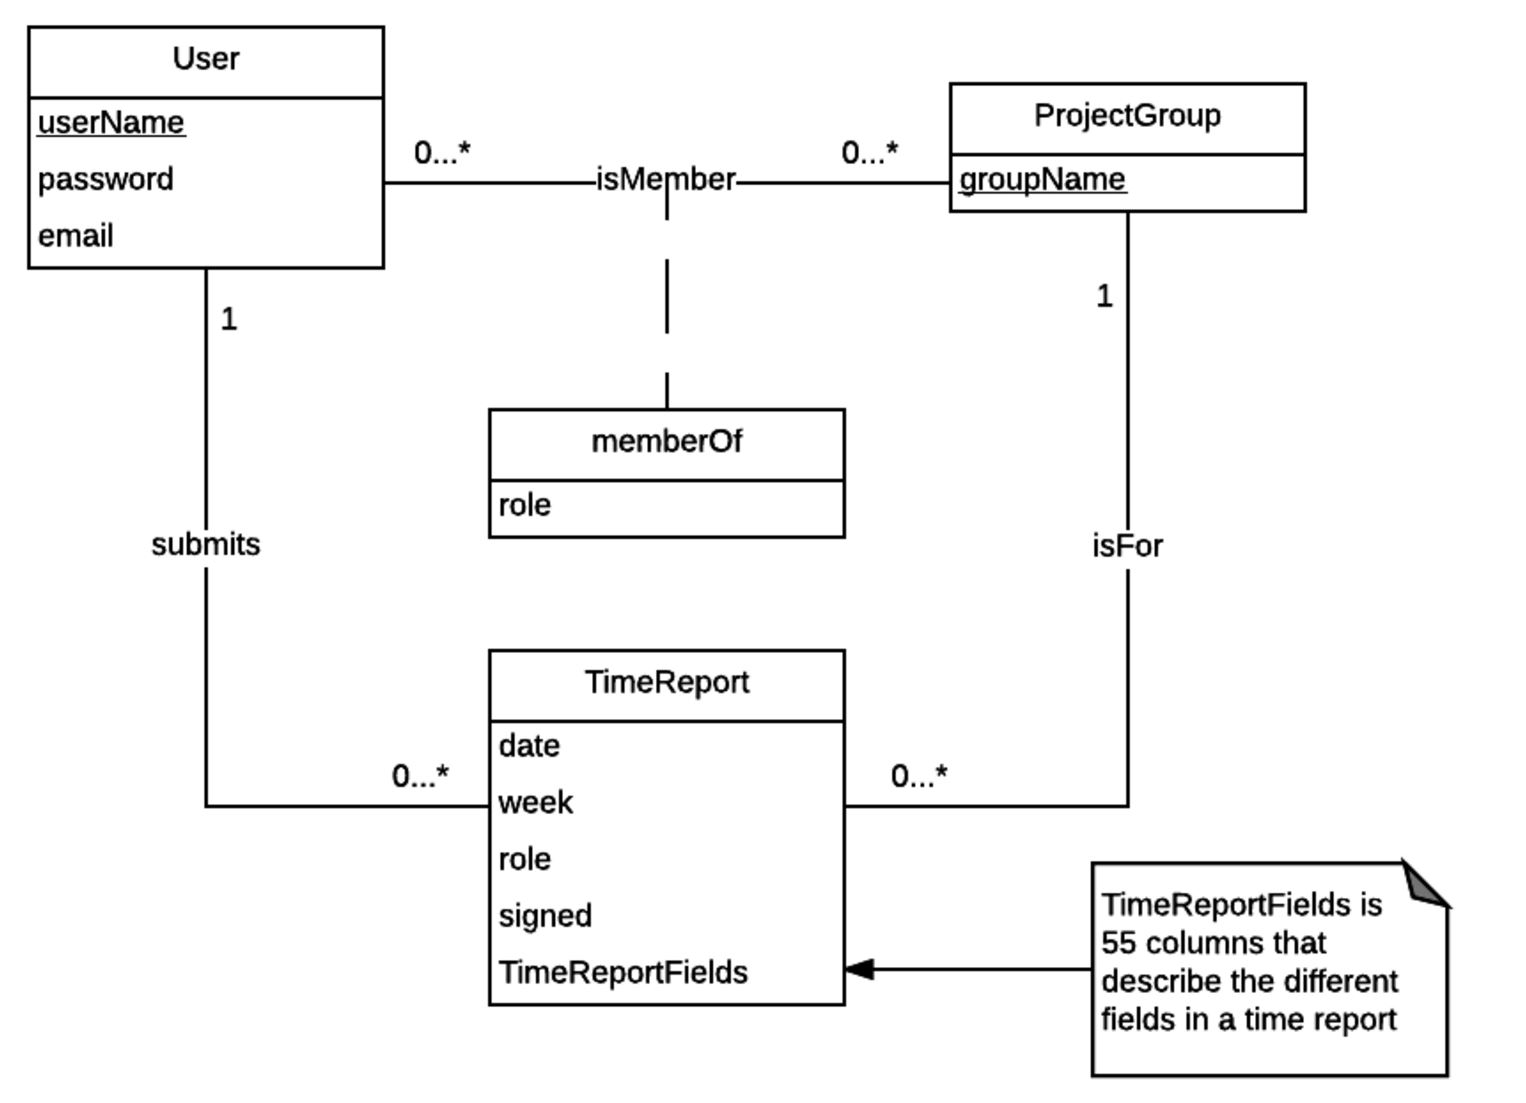
\includegraphics{ERmodel}
\newline
\subsection{Users}

 Users(userName, password, email)
  Users är en tabell som innehåller användare som är inlagda i systemet. Den består av tre    
  kolumner: userName, password och email. userName är primary key vilket innebär att det     
  endast kan finnas en användare med det användarnamnet.\newline
 Tabellen har följande utseende:\newline
\newline
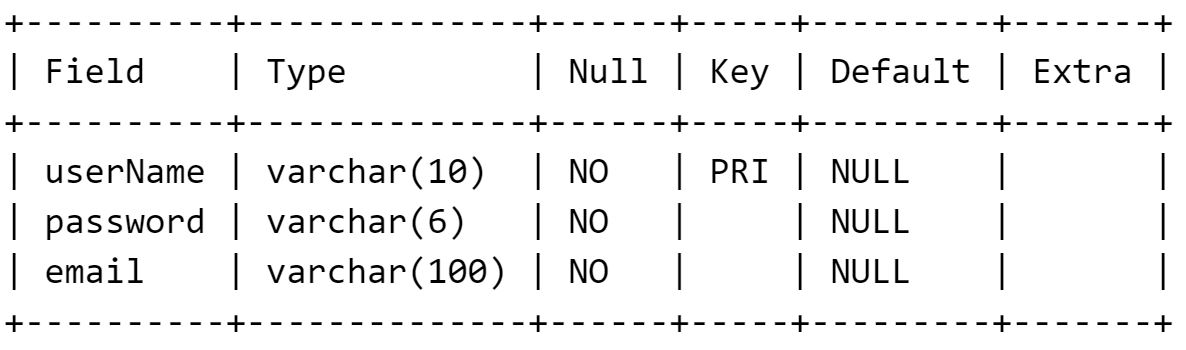
\includegraphics{UsersTable}
\newline
Tabellen kan konstrueras med följande SQL-satser:
\newline
mysql> CREATE TABLE Users (\newline
    -> userName varChar(10) NOT NULL,\newline
    -> password varChar(6) NOT NULL,\newline
    -> email varChar(100) NOT NULL,\newline
    -> PRIMARY KEY (userName));

\subsection{ProjectGroups}
 ProjectGroups(groupName)\newline
   ProjectGroups är en tabell som innehåller de olika projektgrupperna i systemet. Den    
   innehåller endast en kolumn, groupName, som är satt som "primary key" vilket innebär att alla 
   projektgrupper måste ha unika namn.\newline

  Tabellen har följande utseende:
\newline
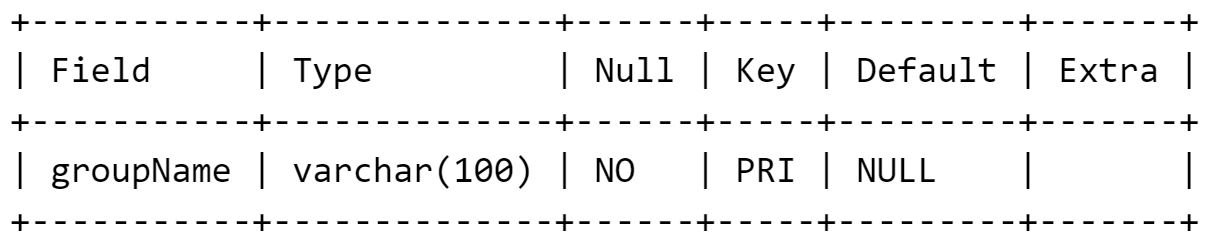
\includegraphics{ProjectGroupsTable}
\newline
\newline
Tabellen kan konstrueras med följande SQL-satser:\newline
mysql> CREATE TABLE ProjectGroups (\newline
    -> groupName varChar(100),\newline
    -> PRIMARY KEY (groupName));

\subsection{TimeReports}
 TimeReports är en tabell som innehåller all information som rör tidrapporterna. Då tabellen 
    har många kolumner (65 st) visas den inte här. För att få ut relevant information ur 
    tidrapporterna så finns det en hjälp-procedure som tar fram relevant information för tillfällen  
    då detta kan kräva många rader kod. För enklare fall så räcker det med en vanlig SELECT.
    Det finns även två triggers, en för när man lägger in en ny rad, och en när man uppdaterar 
    en existerande rad, som väljer rätt roll för användaren, uppdaterar de totala värdena för 
    aktiviteterna med subaktiviteter (11-19), uppdaterar den totala tiden spenderad för 
    subaktiviteterna (d, i, f och r) och den totala tiden rapporten avser.
%%%%Finns inga SQL-satser, eller tabell antagligen för att den var för lång

\subsection{memberOf}
  memberOf(groupName, member, role)\newline
   memberOf är en relationstabell som beskriver relationen mellan användare och de olika 	      
   projektgrupperna. Den har tre kolumner: groupName, member och role. Kolumnerna  
   groupName och member är tillsammans satta som UNIQE, vilket resulterar i att en medlem 
   endast kan vara medlem i samma grupp en gång (en roll per projektgrupp). groupName är en "foreign key" som refererar till \textbf{ProjectGroup(groupName)} och member är en "foreign key" som refererar till \textbf{Users(userName)}.\newline

   Tabellen har följande utseende:\newline
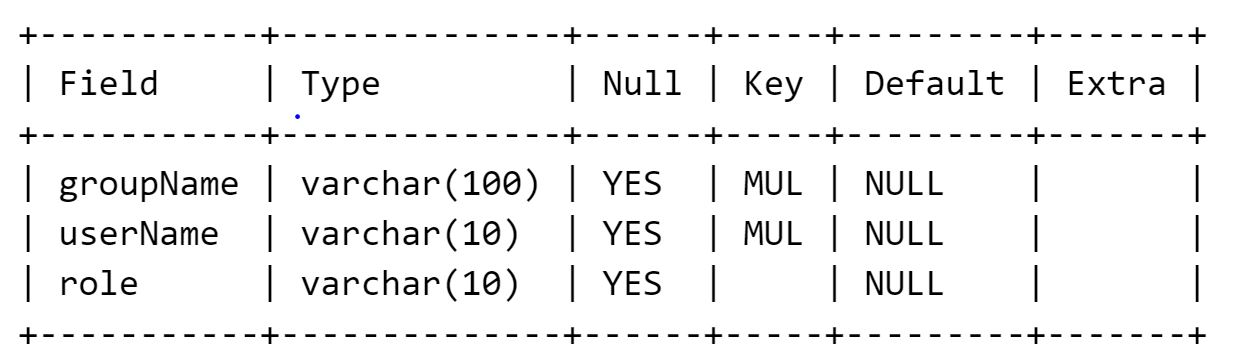
\includegraphics{memberOfTable}
\newline
\newline
Tabellen kan konstrueras med följande SQL-satser:\newline
mysql> CREATE TABLE memberOf (\newline
    -> groupName varChar(100),\newline
    -> member varChar(10),\newline
    -> role varChar(10),\newline
    -> UNIQUE (groupName, member),\newline
    -> FOREIGN KEY (groupName) references ProjectGroups(groupName) ON UPDATE CASCADE\newline
    -> ON DELETE CASCADE,\newline
    -> FOREIGN KEY (member) REFERENCES users(userName) ON UPDATE CASCADE ON DELETE CASCADE);\newline

\section{Klassdiagram}
Ett klassdiagram för Java-klasserna hittas i Appendix A.

\section{Information som lagras i sessionen}

Under varje session lagras följande attribut i sessionen utöver det som redan beskrivs i STLDD:n för BaseBlockSystem:

\textbf{Long lastActive:} 	används för att hålla reda på när användaren senast var aktiv i servern.
\newline
\newline
Följande gäller:
\newline
\textbf{lastActive => 30:}	Användaren har inte varit aktiv i servern under de senaste 30 minuterna och blir därmed utloggad.
	

\textbf{String group:} Gruppnamnet för gruppen användaren valt vid inloggning, tex. ‘Grupp 2’



\section{Sekvensdiagram}
%%kommentarer och sekvensdiagram behöver läggas till
\section{Routing}%%Ska vi ha denna i STLDD:n?

\section{Appendix A}
Klassdiagrammet för Java-klasser. Diagrammet är delat på mitten, så slutstrecket i fig. A.1 fortsätter i fig. A.2.

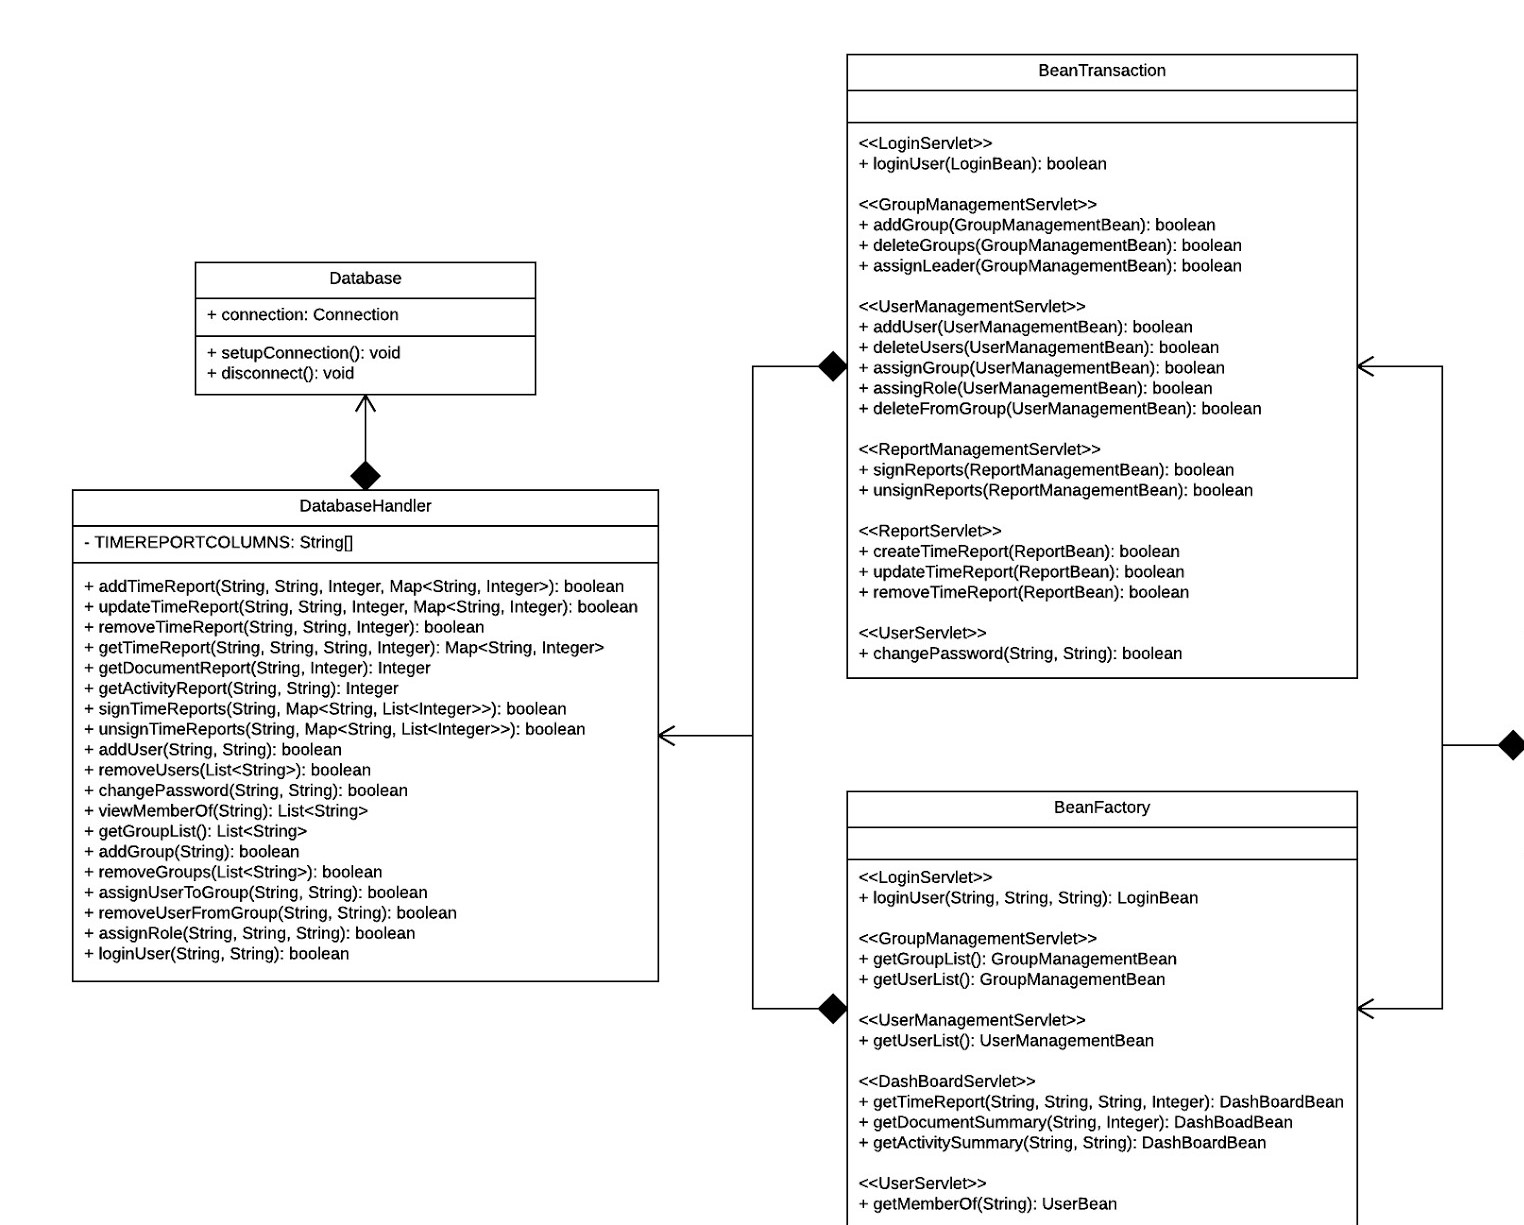
\includegraphics{Klassdiagram1}

Figur A.1. Första halvan i klassdiagrammet.
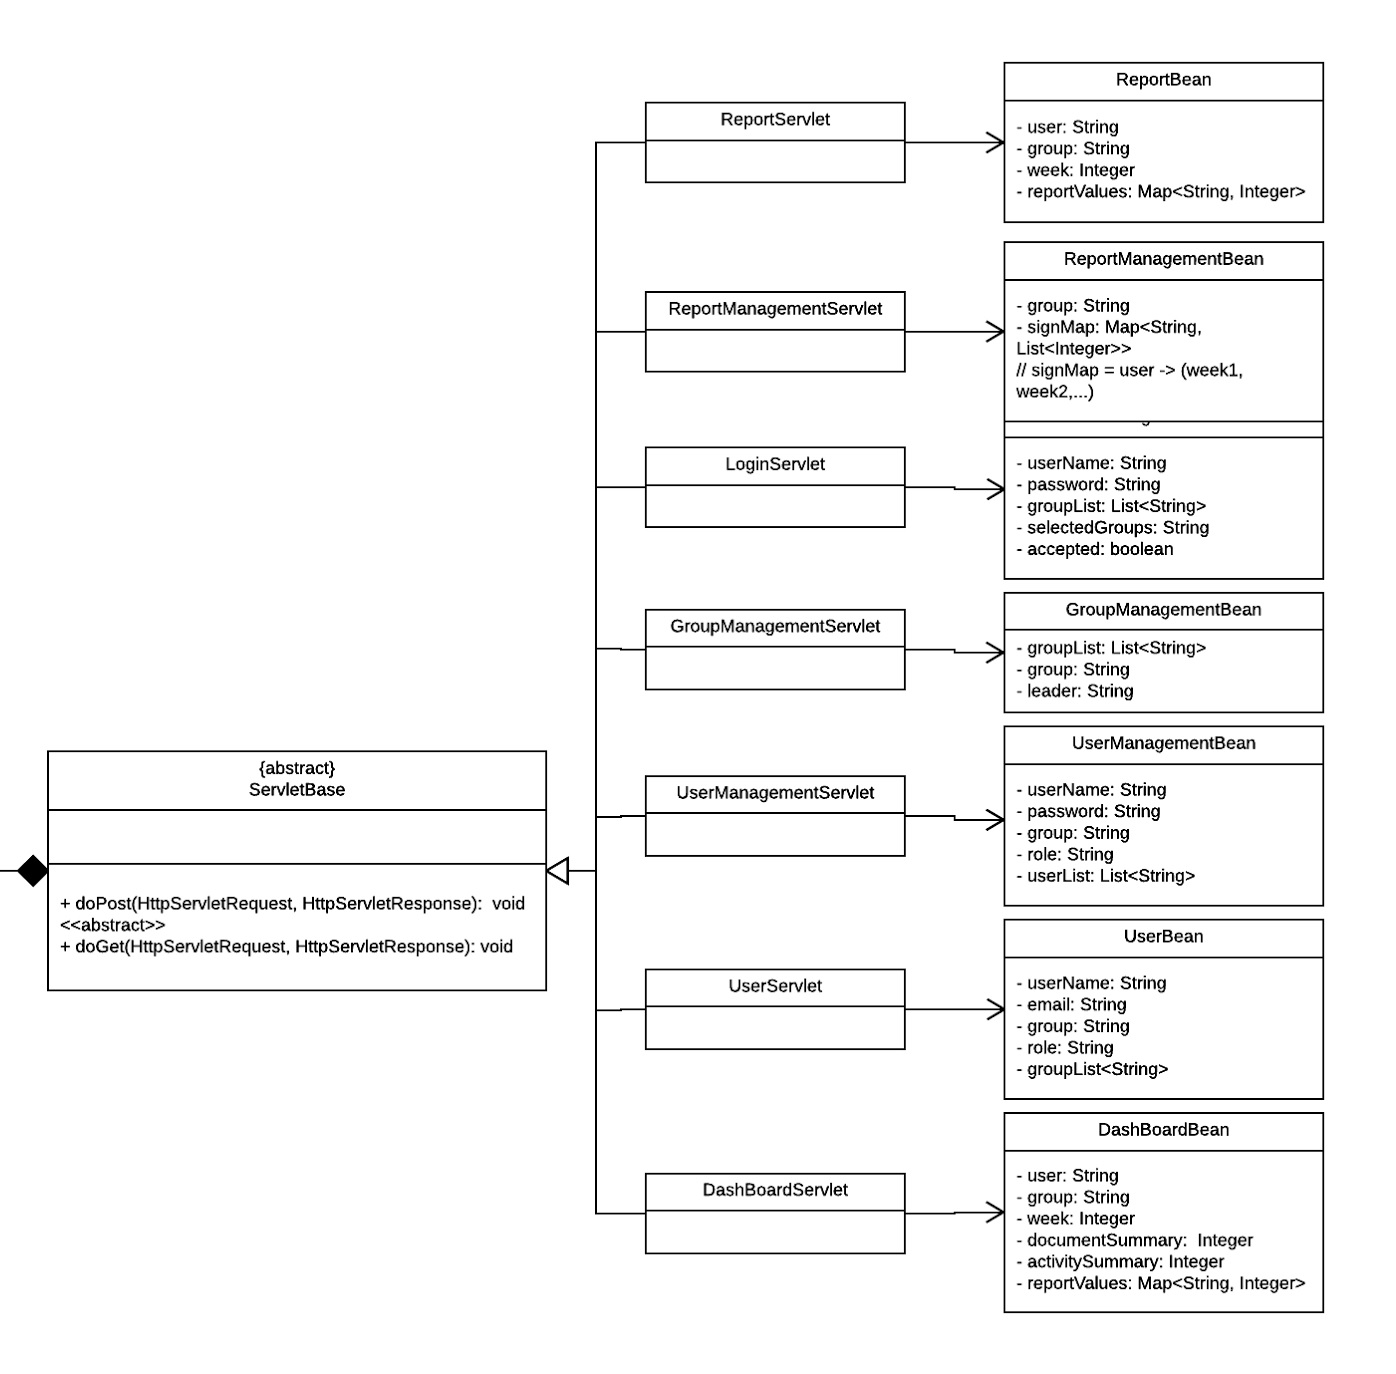
\includegraphics{Klassdiagram2}%%lyckas inte få till denna bild

Figur A.2. Andra halvan i klassdiagrammet.


\end{document}










